\documentclass[a4paper]{article}
\usepackage{tikz}
\usetikzlibrary{shapes.geometric, arrows}
\tikzstyle{startstop} = [ellipse, minimum width=60,text centered, draw=black, fill=red!30]
\tikzstyle{input} = [trapezium, trapezium left angle=110, trapezium right angle=110, minimum width=60, text centered, draw=black, fill=blue!30]
\tikzstyle{output} = [trapezium, trapezium left angle=70, trapezium right angle=70, minimum width=60, text centered, draw=black, fill=blue!30]
\tikzstyle{process} = [rectangle, minimum width=60, text centered, draw=black, fill=orange!30]
\tikzstyle{forinit} = [rectangle, minimum width=60, text centered, draw=black, fill=green!30]
\tikzstyle{decision} = [diamond, shape aspect = 2.5, minimum width=60, text centered, draw=black, fill=green!30]
\tikzstyle{arrow} = [thick, -> ,>=stealth]
\tikzstyle{blank} = [circle, inner sep=0pt, minimum size=3, fill=black]
\begin{document}
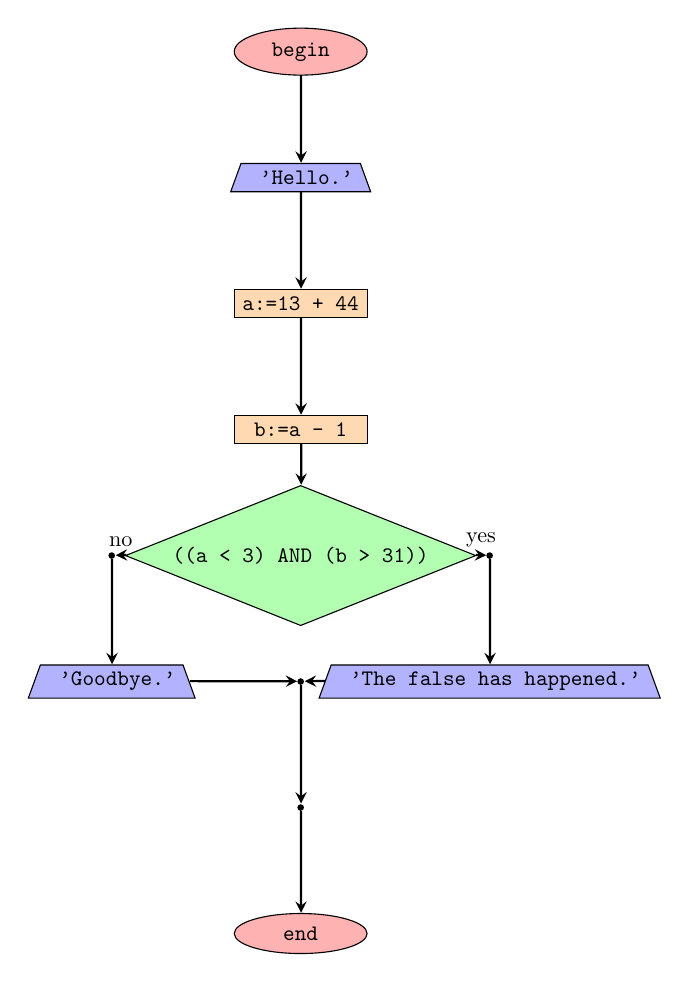
\begin{tikzpicture}[scale=0.8,every node/.style={scale=0.8}]
\node (node0) [startstop] at (100, 100) {\verb|begin|};
\node (node1) [output] at (100, 98) {\verb| 'Hello.' |};
\draw [arrow] (node0) -- (node1);
\node (node2) [process] at (100, 96) {\verb|a:=13 + 44|};
\draw [arrow] (node1) -- (node2);
\node (node3) [process] at (100, 94) {\verb|b:=a - 1|};
\draw [arrow] (node2) -- (node3);
\node (node4) [decision] at (100, 92) {\verb|((a < 3) AND (b > 31))|};
\draw [arrow] (node3) -- (node4);
\node (node5) [blank] at (97, 92) {};
\draw [arrow] (node4) -- node[anchor = south]{no} (node5);
\node (node6) [output] at (97, 90) {\verb| 'Goodbye.' |};
\draw [arrow] (node5) -- (node6);
\node (node7) [blank] at (103, 92) {};
\draw [arrow] (node4) -- node[anchor = south]{yes} (node7);
\node (node8) [output] at (103, 90) {\verb| 'The false has happened.' |};
\draw [arrow] (node7) -- (node8);
\node (node9) [blank] at (100, 90) {};
\draw [arrow] (node8) -- (node9);
\draw [arrow] (node6) -- (node9);
\node (node10) [blank] at (100, 88) {};
\draw [arrow] (node9) -- (node10);
\node (node11) [startstop] at (100, 86) {\verb|end|};
\draw [arrow] (node10) -- (node11);
\end{tikzpicture}
\end{document}
